\chapter{Firefox Add-on Development}

There are two main ways to build Firefox extensions. The traditional way is using XPCOM and XUL. Much of mozilla documentation is focused on XUL add-on, because this has been around for many years. More details about XUL add-on development can be found at [32]. Add-on SDK is the newer kind and was built under Jetpack Project. Jetpack's main agenda is to make it easy to build Firefox add-ons by using HTML, CSS and JavaScript [3].

It is advisable to use the Add-on SDK because of the advantages it provides compared to XUL [33]:

\begin{enumerate}
\item Simplicity: High-level JavaScript APIs provided by SDK like basic user interface components and their functionality simplifies all the common tasks in add-on development. 
\item Compatibility : Electrolysis, also called e10s, is the project under which Firefox is being developed with new multiple process architecture [34]. API's provided by this SDK are designed to be forward-compatible with this new architecture. 
\item Security: It is not easy to build insecure add-ons using the SDK. Even the insecure Add-on that was compromised can do very less damage to the victim's machine.
\item Restartlessness: To install extensions developed using SDK, we no need to restart the browser.
\item Mobile Support: Add-ons can also be developed for the Firefox mobile using the experimental support provided by SDK 1.5
\end{enumerate}

Whereas XUL provides huge number of options for UI when compared to SDK and that's the reason XUL is user for developing add-ons that require rich user interface.

This chapter focuses on important topics of SDK based Add-on development including download and installation of SDK, usage of cfx tool, creation of user interface, interaction with the browser, logging messages to the console for debugging Add-on code and unit testing.

\section{Installation of SDK}

Below softwares are required to build an Add-on:

\begin{enumerate}
\item Make sure that Python 2.5, 2.6 or 2.7 is installed and added to your path. Python 3.x is not supported yet on any platform. 
\item Add-on SDK. Latest stable version of the SDK can be downloaded from the below URLs
\begin{enumerate}
\item \textbf{Tarball file}: https://ftp.mozilla.org/pub/mozilla.org/labs/jetpack/jetpack-sdk-latest.tar.gz
\item \textbf{Zip file}: https://ftp.mozilla.org/pub/mozilla.org/labs/jetpack/jetpack-sdk-latest.zip
\end{enumerate}
\end{enumerate}

\noindent
\textbf{Installation on OS X, Linux, FreeBSD}:

Extract the downloaded SDK file and navigate to the SDK root directory as shown below:

\begin{lstlisting}[frame=none,numbers=none]
tar -xf addon-sdk.tar.gz
cd addon-sdk
\end{lstlisting}

The activate file in bin directory contains instructions to set environment variables required for SDK. To execute this file use the below commands,
\begin{lstlisting}[frame=none,numbers=none]
Bash user: source bin/activate
Whereas non-Bash user: bash bin/activate
\end{lstlisting}


Below is the sample output after executing the activate file,
\begin{lstlisting}[frame=none,numbers=none,mathescape=false]
Sravans-MacBook-Pro:addon-sdk-1.17 sravan2j$ source bin/activate
Welcome to the Add-on SDK. For the docs, visit https://addons.mozilla.org/en-US/developers/docs/sdk/latest/
(addon-sdk-1.17)Sravans-MacBook-Pro:addon-sdk-1.17 sravan2j$ 
\end{lstlisting}


\noindent
\textbf{Installation on OS X using single command}:

Mac user can install the SDK using Homebrew: 
\begin{lstlisting}[frame=none,numbers=none,mathescape=false]
brew install mozilla-addon-sdk
\end{lstlisting}


In this approach, it is not required to execute bin/activate.

\noindent
\textbf{Installation on Windows}:

Extract the downloaded SDK file and navigate to the SDK root directory using command prompt as shown below:
\begin{lstlisting}[frame=none,numbers=none]
7z.exe x addon-sdk.zip
cd addon-sdk
\end{lstlisting}


Then execute the below command to set environment variables required for SDK:
\begin{lstlisting}[frame=none,numbers=none]
bin\activate
\end{lstlisting}


Now, command prompt will be prefixed with SDK's root directory full path:
\begin{lstlisting}[frame=none,numbers=none]
(C:\Users\mozilla\sdk\addon-sdk) C:\Users\Sravan\Desktop\sdk\addon-sdk>
\end{lstlisting}


\noindent
\textbf{Verification of installation}:

To verify the installation of SDK execute the below command in command prompt:
\begin{lstlisting}[frame=none,numbers=none]
cfx
\end{lstlisting}


It should produce output whose first line looks something like this, followed by many lines of usage information:
\begin{lstlisting}[frame=none,numbers=none,mathescape=false]
(addon-sdk-1.17)Sravans-MacBook-Pro:addon-sdk-1.17 sravan2j$ cfx
Usage: cfx [options] command [command-specific options]
\end{lstlisting}

If this kind of information isn`t displayed, then there is a problem with installation.


\section{Initializing an empty add-on}

Create a new directory anywhere in the system and navigate into it, then execute \textbf{cfx init} command as shown below:
\begin{lstlisting}[frame=none,numbers=none,mathescape=false]
(addon-sdk-1.17)Sravans-MacBook-Pro:~ sravan2j$ mkdir sample-addon
(addon-sdk-1.17)Sravans-MacBook-Pro:~ sravan2j$ cd sample-addon/
(addon-sdk-1.17)Sravans-MacBook-Pro:sample-addon sravan2j$ cfx init
\end{lstlisting}

Below is the sample output,

\begin{lstlisting}[basicstyle=\linespread{0.2},frame=none,numbers=none,mathescape=false,upquote=true,keywordstyle=\color{black},stringstyle=\color{black}]
* lib directory created
* data directory created
* test directory created
* generated jID automatically: jid1-oMoaxANUweASVg
* package.json written
* test/test-main.js written
* lib/main.js written
Your sample add-on is now ready.
Do "cfx test" to test it and "cfx run" to try it.  Have fun!
\end{lstlisting}


\textbf{cfx init} command will create a skeleton add-on, as a starting point for add-on development, with the file structure as shown in Figure ~\ref{fig:filestructure}:
\begin{figure}[h]
  \centering
\begin{lstlisting}[frame=single,numbers=none,mathescape=false]
- sample-addon
	- data
	- lib
		- main.js
	- package.json
	- test
		- test-main.js
\end{lstlisting}
    \caption[Add-on file structure]{Add-on file structure example [1].}
    \label{fig:filestructure}
\end{figure}
\section{Implementing the sample add-on}

Add-on code should be written in "main.js" file inside lib directory. Include the code in Figure~\ref{fig:sampleaddon}, into main.js file [1],

\begin{figure}[h]
  \centering
\begin{lstlisting}[language=JavaScript]
var buttons = require("sdk/ui/button/action");
var tabs = require("sdk/tabs");

var button = buttons.ActionButton ({
  id: "mozilla-url",
  label: "Visit Mozilla",
  icon: {
    "16": "./icon-16.png",
    "32": "./icon-32.png",
    "64": "./icon-64.png"
  },
  onClick: handleClick
});

function handleClick(state) {
  tabs.open("https://www.mozilla.org/");
}
\end{lstlisting}
    \caption[Sample add-on code]{Sample add-on code [1].}
    \label{fig:sampleaddon}
\end{figure}

Download the below Mozilla icon files and save them in "data" directory:
\begin{enumerate}
\item icon-16.png : https://mdn.mozillademos.org/files/7635/icon-16.png
\item icon-32.png : https://mdn.mozillademos.org/files/7637/icon-32.png
\item icon-64.png : https://mdn.mozillademos.org/files/7639/icon-64.png
\end{enumerate}
Then execute the following command to run a new instance of Firefox browser with the newly developed add-on installed:
\begin{lstlisting}[frame=none,numbers=none,mathescape=false]
cfx run
\end{lstlisting}
When the browser launches, there will be an icon with Firefox logo in the top-right corner of browser as shown in Figure ~\ref{fig:mozilla-button}. Clicking this icon will open a new tab with https://www.mozilla.org/ loaded into it.
\begin{figure}[h]
  \centering
      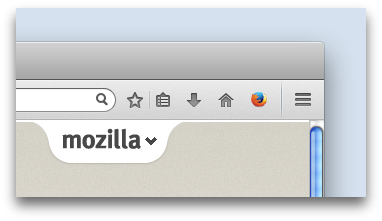
\includegraphics[width=8cm, height=4.6cm]{mozilla-button.png}
    \caption[Add-on with firefox logo]{Add-on with firefox logo [20].}
    \label{fig:mozilla-button}
\end{figure}

\section{Packaging the add-on}

After developing an Add-on, we need to package it as an XPI file for distribution. XPI is the installable file format for add-ons. We can distribute this XPI files or we can publish the add-ons in https://addons.mozilla.org, so that users can download and install them.

To build an XPI, just execute the command cfx xpi from the add-on's directory:
\begin{lstlisting}[frame=none,numbers=none,mathescape=false]
cfx xpi
\end{lstlisting}


After executing the command, a new file like "sample-addon.xpi" will be created in the directory. This ".xpi" file can be installed in Firefox as follows:
\begin{enumerate}
\item Select the "Open" item from Firefox's "File" menu.
\item Navigate to the "sample-addon.xpi" file and open it. A prompt will be displayed to install add-on as shown in Figure ~\ref{fig:install}. Follow the instructions to install the add-on.
\end{enumerate}

\begin{figure}[h]
  \centering
      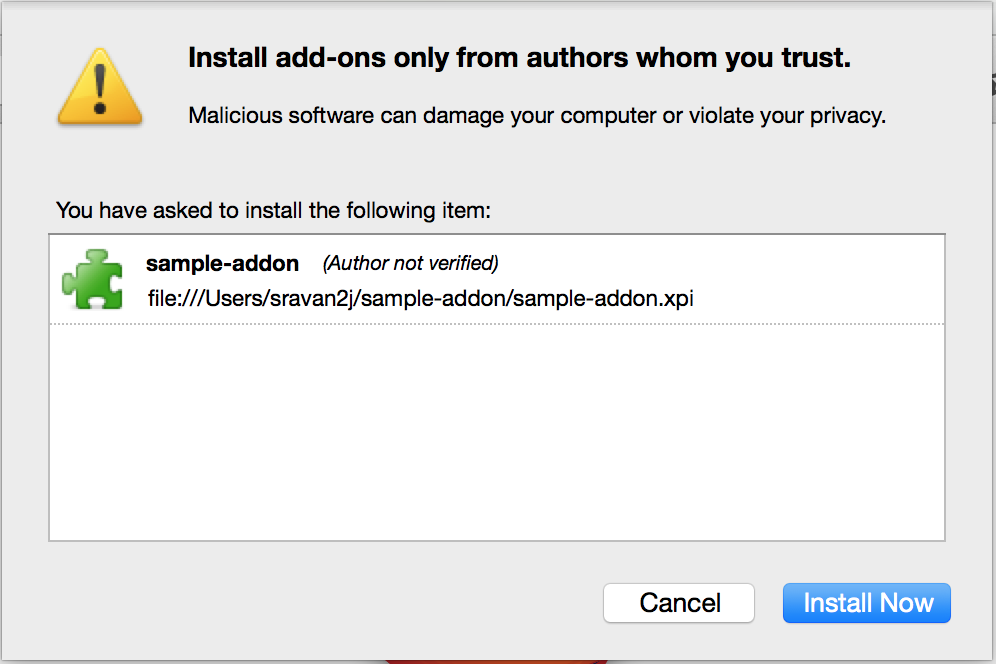
\includegraphics[width=10cm, height=6.6cm]{install.png}
    \caption[Add-on with firefox logo]{Add-on with firefox logo [20].}
    \label{fig:install}
\end{figure}

\section{Logging}

Generally, JavaScipt code is debugged using DOM console object but DOM objects aren't available to the add-on code, so a global "console" object was provided by the SDK. SDK's console object has almost the same methods as the DOM console object, including methods to log warning, error or informational messages. console object is automatically available to the add-on code, we no need to require() anything.

The console.log() method is used to display informational message:
\begin{lstlisting}[frame=none,numbers=none,language=JavaScript]
console.log("Hello World");
\end{lstlisting}
If the add-on was executed from the command line using "cfx run". Then the above instruction outputs the below message in the command shell used to run add-on:
\begin{lstlisting}[frame=none,numbers=none]
info: Hello World!
\end{lstlisting}
\section{Open a Web Page}

open() method of tabs module is used to open a new webpage and before using this command, we need to import "tabs" module using require() command. For instance, line 1 and 3 of the code in Figure ~\ref{fig:sampleaddon}, corresponds to opening a new web page.

\section{Creating buttons}

To create a button we must provide an ID, an icon and a label to the button as shown in lines 4-13 of the code in Figure ~\ref{fig:sampleaddon}

Instruction 1 of the code in Figure ~\ref{fig:sampleaddon}, shows how to import action module of the button. As I mentioned earlier, a module needs to be imported before making use of any function in that module.

\section{Listen for Page Load}

Tabs object has built-in ready event which can be used to listen for the web page load. Figure ~\ref{fig:pageload} contains the code that logs web page url as the user loads the page [1].
\begin{figure}[h]
  \centering
\begin{lstlisting}[language=JavaScript]
require("sdk/tabs").on("ready", logURL);

function logURL(tab) {
  console.log(tab.url);
}
\end{lstlisting}
    \caption[Add-on code that listens for page load]{Sample add-on code that listens for Page Load [1].}
    \label{fig:pageload}
\end{figure}

\section{File i/o}

File module provided by the SDK is used to access the local filesystem. Below are some of the important methods in File module
\begin{description}
\item[exists(filepath)]\hfill \\
Returns true if the file denoted by the filepath exists and false otherwise.
\item[list(path)]\hfill \\
Returns an array of files exists in the given path.
\item[mkpath(path)]\hfill \\
Creates a new directory denoted by the given path. If any subdirectories do not exist, then this sub directories also be automatically created.
\item[open(filepath, mode)]\hfill \\
Returns a stream providing access to the file contents. Filepath parameter species the file to open. Below are the acceptable values for mode parameter:
\begin{enumerate} 
\item "r" - If the file is to be opened in read-only mode. This is the default value. 
\item "w" - If the file is to be opened in write-only mode 
\item "b" - If the file is to be opened in binary mode 
\end{enumerate}
\item[read(filepath, mode)]\hfill \\
Opens a file specified by filepath and then return the file contents as a string.
\item[remove(filepath)]\hfill \\
Removes a file from the file system. 
\item[rmdir(path)]\hfill \\
Removes a directory specified by the path. If the directory is not empty then the method throws an exception.
\item[isFile(filepath)]\hfill \\
Returns true if the filepath specifies a file.
\end{description}


Code in Figure~\ref{fig:fileioaddon}, checks what all files and directories present in "/Users/Work/" directory and display this information.
\begin{figure}[h]
  \centering
\begin{lstlisting}[language=JavaScript]
const fileIO = require("sdk/io/file");

let path = "/Users/Work/";
let list = fileIO.list(path);

for (i = 0; i < list.length; i++) {
  let item = fileIO.join(path, list[i]);
  if (fileIO.isFile(item)) {
    console.log(item + " is a file");
  }
  else {
    console.log(item + " is a directory");
  }
}
\end{lstlisting}
    \caption[Sample file i/o add-on code]{Sample file i/o add-on code [1].}
    \label{fig:fileioaddon}
\end{figure}

\section{Communicating using "port"}

Add-on's main code, including "main.js" and other modules in "lib", can use the SDK high-level and low-level APIs, but can't access web content directly. Whereas content scripts can't use the SDK's APIs but can access web content.

So if incase when we have to build an Add-on which works based on the content of the web page, then we have to make use of the content scripts to access the web page contents.

Content scripts are placed in data subdirectory.


\textbf{Loading content scripts:}


Single content scripts can be loaded by assigning a string to either the \textbf{contentScript} or the \textbf{contentScriptFile} option as shown in Figure~\ref{fig:loadingcs}.
\begin{figure}[h]
  \centering
\begin{lstlisting}[language=JavaScript]
var pageMod = require("sdk/page-mod");

pageMod.PageMod({
  include: "*.mozilla.org",
  contentScriptFile: "./content-script.js"
});
\end{lstlisting}
    \caption[Loading content scripts example]{Loading content scripts example [1].}
    \label{fig:loadingcs}
\end{figure}


We can load multiple content scripts by passing an array of files to \textbf{contentScriptFile} as shown below:
\begin{lstlisting}[frame=none,numbers=none,language=JavaScript]
contentScriptFile: [ "./content-script1.js", "./content-script2.js" ]
\end{lstlisting}


\textbf{Communicating with the add-on:}

To enable add-on scripts and content scripts to communicate with each other, each end of the conversation has access to a port object.
\begin{enumerate}
\item port.emit() is used to send messages from one side to the other 
\item port.emit() is used to receive messages sent from the other side
\end{enumerate}

\begin{figure}
  \centering
      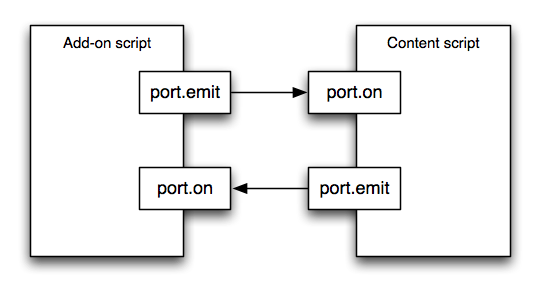
\includegraphics[width=16cm, height=8.65cm]{content-scripting-overview.png}
    \caption[Communication among add-on and content script]{Communication among add-on and content script [1].}
    \label{fig:content-scripting-overview}
\end{figure}

Messages are asynchronous i.e., after sending the message, sender continues processing without waiting for a reply from the recipient.

Add-on code in Figure~\ref{fig:communication}, adds a button to Firefox. When the user clicks this button, add-on attaches a content script to the active tab, sends the \textbf{addon-message} to content script. When content script receives add-on message, it will retrieve the first paragraph from the loaded web page and send it to add-on along with \textbf{script-response} message. As soon as the add-on receives response from content script, it logs the first paragraph.

\begin{figure}[h]
  \centering

\begin{lstlisting}[language=JavaScript] 
//main.js
var tabs = require("sdk/tabs");
var buttons = require("sdk/ui/button/action");
var self = require("sdk/self");

buttons.ActionButton({
  id: "attach-script",
  label: "Attach the script",
  icon: "./icon-16.png",
  onClick: attachScript
});

function attachScript() {
  var worker = tabs.activeTab.attach({
    contentScriptFile: self.data.url("content-script.js")
  });
  worker.port.on("script-response", function(response) {
    console.log(response);
  });
  worker.port.emit("addon-message", "Message from the add-on");
}
\end{lstlisting}
\begin{lstlisting}[language=JavaScript] 
// content-script.js
self.port.on("addon-message", getFirstPara);

function getFirstPara() {
  var paras = document.getElementsByTagName("p");
  if (paras.length > 0) {
    var firstPara = paras[0].textContent;
    self.port.emit("script-response", firstPara);
  }
}
\end{lstlisting}
    \caption[Communication among add-on and content script using code]{Communication among add-on and content script using code [1].}
    \label{fig:communication}
\end{figure}

\section{Unit Testing}

"\textbf{cfx test}" runs all the unit tests of an add-on. If the "cfx test" command is executed in the add-on's root directory, cfx will:
\begin{enumerate}
\item retrieve the details of tests directories from "tests" value inside "package.json" file. If incase "tests" parameter is not present in package.json, then the top-level "tests/" or "test/" directory is considered as tests directory.
\item load every module present in the tests directory whose file name starts with "test"
\item call each function exported by that module, passing it a test object as an argument.
\end{enumerate}

Assert module is used to implement unit tests. Code in Figure~\ref{fig:unittesting} has one test case which checks whether the value of a is 1 or not. Include this code in test/test-main.js [1]:

\begin{figure}[h]
  \centering

\begin{lstlisting}[language=JavaScript] 
var a = 1;

exports["test value of a"] = function(assert) {
  assert.ok(a == 1, "test that a is 1");
}

require("sdk/test").run(exports);
\end{lstlisting}
    \caption[Sample unit testing code]{Sample unit testing code [1].}
    \label{fig:unittesting}
\end{figure}
Now, execution of "cfx test" command in the add-on's root directory will display the below output,
\begin{lstlisting}[frame=none,numbers=none,mathescape=false]
(addon-sdk-1.17)Sravans-MacBook-Pro:sample-addon sravan2j$ cfx test
Using binary at '/Applications/Firefox.app/Contents/MacOS/firefox-bin'.
Using profile at '/var/folders/y8/w18vnqyx6492t30xqhgffgc80000gn/T/tmpZ51Npa.mozrunner'.
Running tests on Firefox 36.0.4/Gecko 36.0.4 ({ec8030f7-c20a-464f-9b0e-13a3a9e97384}) under darwin/x86_64.
.
1 of 1 tests passed.
Total time: 2.282716 seconds
Program terminated successfully.
\end{lstlisting}
